\usetikzlibrary{arrows,positioning}
\section{Fachlicher Soll-Zustand}


\subsection{Hauptaufgaben der neuen Lösung}

\begin{tabularx}{\textwidth}{| p{0.7cm} | p{1.5cm} | X |}
\hline
\rowcolor[gray]{0.9} Ziel ID & Aufgaben ID & Beschreibung \\
\hline
Z1 & A1 & Es muss ein Tron-Klon programmiert werden welcher über die wichtigsten Funktionen verfügt und es zwei Spielern erlaubt sich gegenseitig zu messen.\\
\hline
Z2.1 & A2.1 & Das Spiel wird um computergesteuerte Gegner ergänzt, welche sich an simple Regeln halten. \\
\hline
Z2.2 & A2.2 & Die Gegner erhalten die Fähigkeit sich dem Spieler anzupassen. \\
\hline 
Z2.3 & A2.3 & Es wird ein Trainings-Mode für die Gegner programmiert welcher es ohne menschliches Einwirken ermöglich bessere Gegner zu trainieren. \\
\hline
Z3 & A3 & Der Trainings-Mode wird erweitert so das es dem Spieler zur verfügung steht mehrere Gegner gezielt zu trainieren, im Trainings-Mode oder gegen den Spieler. \\
\hline
Z4 & A4 & Das Spiel wird über eine Import-Export Funktion verfügen um gegen computergesteuerte Gegner von anderen Spielern zu spielen. \\
\hline
\end{tabularx}

\subsection{Theoretische Umsetzung}

Hier werden die bereits absehbaren Klassen abgebildet. Es soll ein kleiner Überblick darüber bieten wie DARWIN implementiert wird. %insert class diagramm and picture of poc
\\
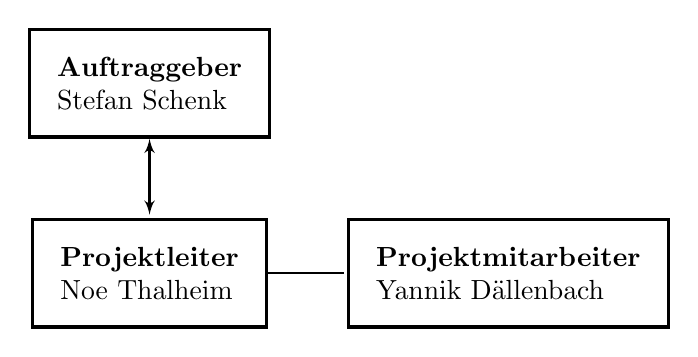
\begin{tikzpicture}[node distance=1cm, auto]  
\tikzset{
	    mynode/.style={rectangle,align=left,draw=black, top color=white, bottom color=white!50,very thick, inner sep=1em, minimum size=3em, text centered},
	    myarrow/.style={->, >=latex', shorten >=1pt, thick},
	    mylabel/.style={text width=7em, text centered} 
	}  
	\node[mynode] (auftraggeber) {\textbf{Auftraggeber}\\Stefan Schenk};  
	\node[mynode, below=1cm of auftraggeber] (projektleiter) 		{\textbf{Projektleiter}\\Noe Thalheim};  
	\node[mynode, right=of projektleiter] (projektmitarbeiter1) 		{\textbf{Projektmitarbeiter}\\Yannik Dällenbach};


	\draw[myarrow] [<->] (auftraggeber.south) -- (projektleiter.north);	
	\draw[myarrow] [-] (projektleiter.east) -- (projektmitarbeiter1.west);

\end{tikzpicture} 
	\medskip

